\documentclass{article}
\usepackage[textwidth=5.5in,textheight=9in]{geometry}
\usepackage{amsmath,booktabs,hyperref,graphicx}
\title{Experimental text for draft integration}
\author{}
\date{September 14, 2026}
\begin{document}
\maketitle
% Insert into the supplied draft before its AI-use statement.
% Tables are in paper_results.tex; paths may be adjusted when copying files.
\section{Experiments}
\label{sec:experiments}

We distinguish two questions. First, does conditioning the actual frozen policy
on feasibility improve useful behavior relative to projecting its samples?
Second, does a finite implementation of our refinement mechanism recover those
benefits and approximate the conditional distribution? These questions need
separate controls: improved return alone does not establish conwhaditional sampling.

\paragraph{Controlled protocol.}
Let $p_{\mathrm{sampler}}(A\mid s)$ denote the distribution produced by the
frozen 100-step DDPM, including normalization and physical action clipping.
Our reference returns the first feasible independent proposal, without ranking
accepted proposals by reward. It samples the feasible conditional law given
budget success. All proposals and budget failures are retained. Projection
minimizes squared Euclidean distance over the same complete action chunk and
feasible set. Every method receives the same observation and constraints,
executes the same chunk duration, and then uses the same deterministic public
RL controller. We measure unchanged native return, feasibility, failures,
boundary concentration, action-kernel discrepancy, and cost.

We evaluate Pendulum with a 0.6 s chunk and 10 s total rollout, using mirrored
initial torque envelopes $[-2,0]^{12}$ and $[0,2]^{12}$. Walker2d and HalfCheetah
use 0.096 s and 0.4 s chunks respectively, followed by continuation through
4 s total. Their feasible sets intersect the physical action box with a
whole-chunk RMS actuator-command budget. These convex constraints admit
global projection: coordinate clipping for Pendulum and the scalar KKT
solution for a box intersected with a Euclidean ball. The RMS envelope is
an effort proxy applied to the initial chunk; it does not certify subsequent
state safety or measure mechanical energy.

Pendulum uses 64 held-out states and 8 replicates per state. Each MuJoCo task
uses 32 full simulator snapshots and 4 replicates; half are reset states and
half follow 1 s of expert warmup. Observations, model weights, constraints,
seeds, horizons, and analysis rules were frozen before evaluation. Rejection
budgets are 64 proposals per Pendulum request and 128 per MuJoCo request.
State-cluster bootstrap intervals account for repeated samples from one state.
The new Pendulum baseline comparisons use a four-comparison correction;
MuJoCo's two primary contrasts at four settings use an eight-comparison
correction. These intervals condition on the trained policies and do not
estimate variation across independent training runs.

\paragraph{Policies and finite samplers.}
The Pendulum DDPM imitates complete episodes from a public TD3 controller and
its reflected counterpart. For each MuJoCo task, we acquired released
Farama-Minari SAC expert and medium controllers and collected 128 complete
episodes from 64 paired reset groups. Groups were split 48/8/8 before
overlapping action chunks were constructed, and observation normalization used
training episodes only. Initial diffusion fits failed the development quality
gate. A single bounded refit shortened Walker2d's chunk and increased
early-episode sampling; both resulting policies passed the gate before safety
comparisons. All initial fits and failed outcomes are retained.

Our finite sampler uses $\gamma=1/2$ and an annealed refinement schedule with
256, 256, and 512 updates at DDPM indices 20, 5, and 0. The VP epsilon network
is converted to a VE score at each level. Within each level,
$\alpha_k=0.15\sigma^2/(1+k/64)^{0.6}$. This is a finite annealed variant,
not a test of all relaxation parameters or of asymptotic convergence.

We additionally compare a paper-derived DDPM reimplementation of BayesFP
(\href{https://arxiv.org/abs/2606.21014}{Sirigiri et al., 2026}), using 32 particles and a safety-only
cost. Guidance strength is selected by development discrepancy from rejection,
without optimizing task reward. We report both raw output and output followed
by the identical exact projection. The latter is the hard-feasible comparison.
Pendulum also includes 12 particles, approximately matching our score count.
This is not a reproduction using official author code or author benchmarks.

\input{paper_results.tex}

\paragraph{When conditioning helps.}
Pendulum provides the clearest mechanism: projecting the excluded swing
direction concentrates samples near zero torque, delaying useful motion.
Conditioning improves native return by 56.37 and 47.77 points in the two
mirrored cases; finite refinement improves it by 57.04 and 47.65 points.
Projection places 64.6\% and 65.4\% of outputs on the added zero-torque
boundary, compared with zero observed added-boundary outputs for rejection
and refinement. All methods eventually stabilize in this evaluation; the
improvement is in continuous return and stabilization time, not a higher
completion count. Each signed constraint predominantly retains one useful
direction, so this experiment does not establish preservation of weights among
multiple surviving safe modes.

The effect is task dependent. On Walker2d, conditioning slightly reduces
return relative to projection at both effort caps. On HalfCheetah the
conditioning--projection differences are inconclusive. The earlier released
Push-T policy experiment also failed to produce a useful conditioning gain:
at its stricter reported cap the native coverage difference favored projection.
Thus boundary concentration alone does not establish a meaningful task loss.

\paragraph{Comparison with BayesFP and approximation limits.}
On Pendulum, refinement has no useful return advantage over repaired BayesFP.
For HalfCheetah at RMS cap 0.72, refinement exceeds repaired BayesFP by 30.61
points, with an adjusted interval $[5.44,57.42]$. Its point estimate exceeds
the preregistered 26.19-point useful-effect threshold, while the interval still
allows smaller effects. Conditioning does not outperform projection in this
setting, and refinement's advantage over ordinary projection is inconclusive.
This result therefore supports a finite-sampler comparison, not a causal claim
that more accurate conditioning produced the gain. Walker2d's positive
refinement--BayesFP difference at the stricter cap is below its useful-effect
threshold; one refinement rollout at the milder cap terminates unhealthy.

Raw 32-particle BayesFP violates the chunk constraint in 13.9--18.0\% of
Pendulum outputs and 18.0--57.8\% of MuJoCo outputs. Rejection, projection,
refinement and repaired BayesFP have zero observed chunk violations; rejection
has zero budget failures. Finite refinement remains detectably different from
the rejection reference. In the HalfCheetah setting above, its action-kernel
MMD is 0.157, versus 0.119 for repaired BayesFP and 0.113 for independent
rejection samples. These are finite-sample diagnostics, not calibrated tests
of distributional equality. Recorded batch latency favors BayesFP despite its
larger score count. We therefore do not claim superior online efficiency,
exact conditional sampling, or universal task-quality improvement.

\paragraph{Reproducibility.}
All experiments ran in simulation on the inspected Threadripper 9980X and
RTX 5070 Ti workstation. The artifact includes frozen dependency records,
public asset URLs/revisions/hashes, episode splits, all proposal banks,
complete outcomes including failures, solver checks, simulator replay checks,
and scripts that regenerate tables and figures. A fresh-directory rerun of
HalfCheetah reproduces the saved numerical arrays exactly; this is a
reproducibility check rather than independent statistical evidence.

\clearpage
\begin{figure}[p]
\centering
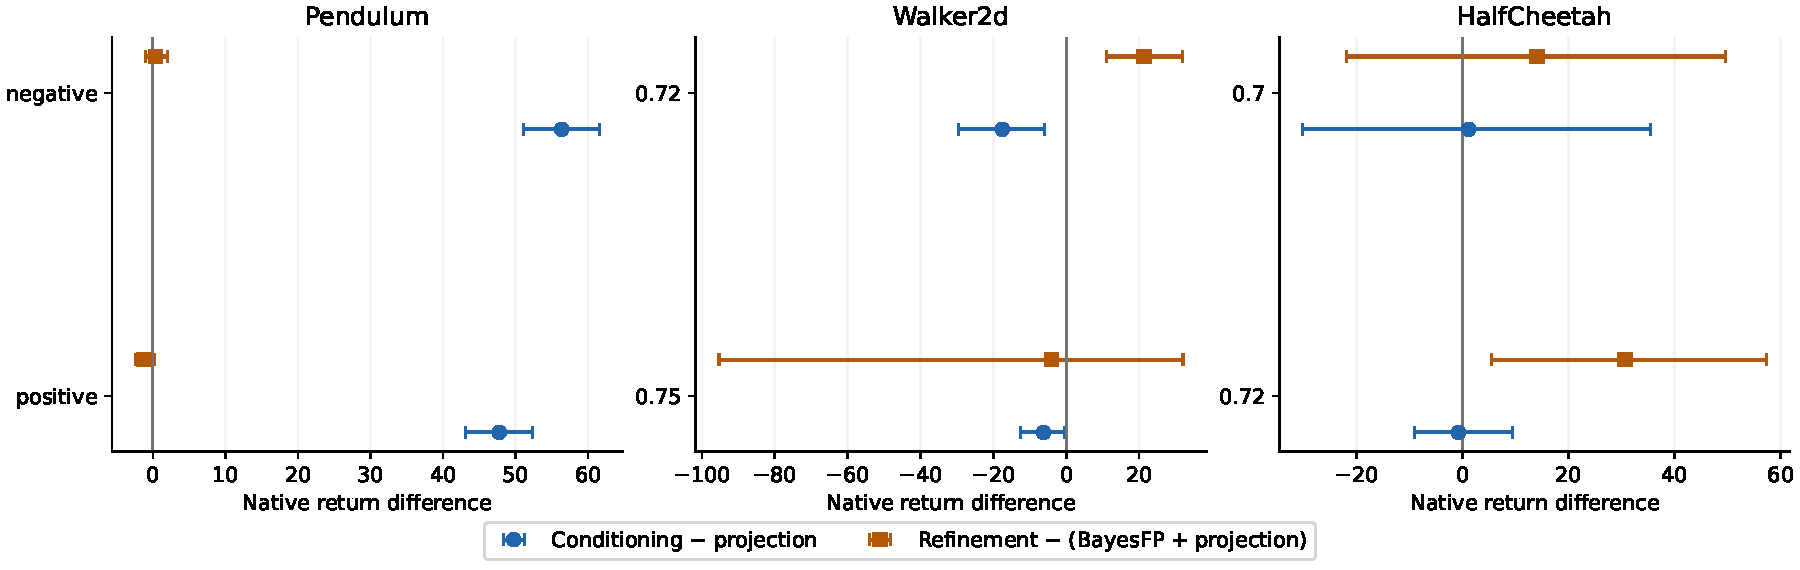
\includegraphics[width=\linewidth]{figures/return_comparisons.pdf}
\caption{Target utility and finite-sampler performance are separate comparisons.
The horizontal axes use each task's native return units. Q--P intervals are
95\% for Pendulum and 99.375\% for MuJoCo; R--(B+P) intervals are 98.75\%
and 99.375\%, respectively. They follow the separate predeclared comparison
families described in the text.}
\end{figure}
\begin{figure}[p]
\centering
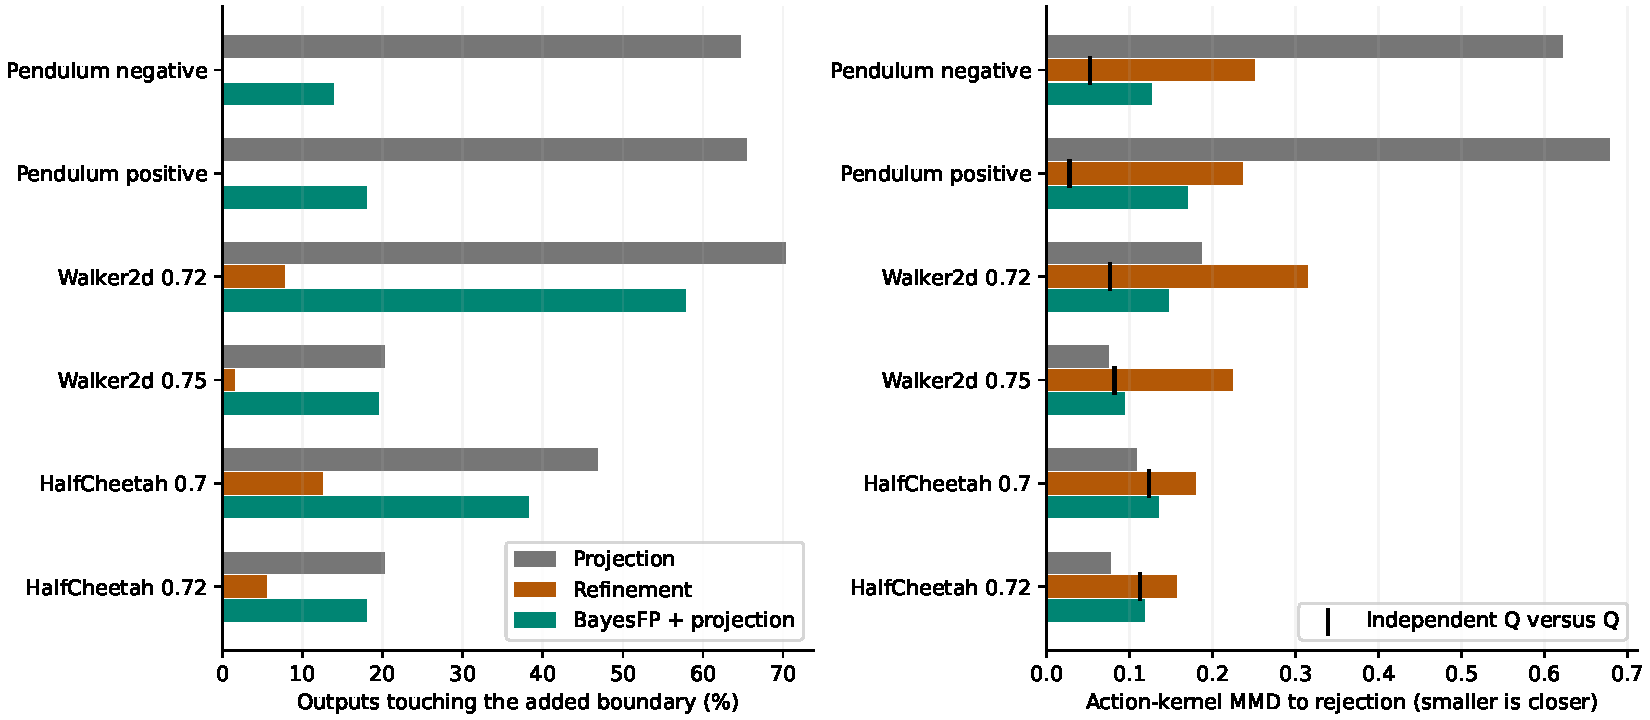
\includegraphics[width=\linewidth]{figures/distribution_diagnostics.pdf}
\caption{Boundary concentration and finite-sample action-kernel discrepancy.
The independent Q-versus-Q marker indicates sampling noise, not a formal
threshold. Kernel RMS bandwidth is .1 for normalized Pendulum actions and
.2 for MuJoCo actions. MMD values therefore should not be compared directly
across tasks. The added safety boundary is distinct from pre-existing physical
action saturation.}
\end{figure}
\end{document}
